\documentclass[a4paper, 12pt]{ctexart}
\setlength{\parindent}{2em}
\usepackage[
  a4paper,
  scale=0.78
]{geometry}
\usepackage{titlesec}
\usepackage{amsmath}
\usepackage{amssymb}
\usepackage{array}
\usepackage{booktabs}
\usepackage{graphicx}
\usepackage{float}
\usepackage[labelsep=period]{caption}
\usepackage{fvextra}
\usepackage{fancyhdr}
\usepackage{tabularx}
\usepackage[colorlinks=true, linkcolor=black, urlcolor=blue]{hyperref}

\setlength{\tabcolsep}{10pt}
\graphicspath{{figures/hw12/}}
\newcommand{\Ts}{T_{\mathrm{s}}}
\newcommand{\Udc}{U_{\mathrm{dc}}}

\titleformat{\section}
  {\normalfont\bfseries\Large}
  {\thesection}{0.8em}{}
\titlespacing{\section}{0pt}{18pt}{8pt}

\titleformat{\subsection}
  {\normalfont\bfseries\large}
  {\thesubsection}{0.8em}{}
\titlespacing{\subsection}{0pt}{12pt}{6pt}

\fvset{
  fontsize=\scriptsize,
  frame=single,
  numbers=left,
  numbersep=6pt,
  breaklines=true,
  tabsize=4
}

\pagestyle{fancy}
\fancyhf{}
\cfoot{{\footnotesize\thepage}}
\renewcommand{\headrulewidth}{0pt}
\renewcommand{\footrulewidth}{0pt}
\fancypagestyle{plain}{
  \fancyhf{}
  \cfoot{{\footnotesize\thepage}}
  \renewcommand{\headrulewidth}{0pt}
  \renewcommand{\footrulewidth}{0pt}
}

\begin{document}

\begin{center}
  {\zihao{3}\bfseries SVPWM 六扇区作用时间推导与仿真}
\end{center}

\vspace{1em}

\tableofcontents
\clearpage

\section{坐标系与坐标变换}

\subsection{ABC 自然坐标系}

三相逆变器的输出电压最先定义在定子三相自然坐标系中。设三相相轴为 $A$、$B$、$C$，且三者在空间中互差 $120^\circ$ 电角度。若以电机定子虚拟中性点 $N$ 为参考，则三相相电压可写为
\[
  \boldsymbol u_{abc}
  =
  \begin{bmatrix}
    u_a \\ u_b \\ u_c
  \end{bmatrix}.
\]

对于三相三线制系统，零序分量不参与电机电磁能量转换，因此有
\[
  u_a + u_b + u_c = 0.
\]
因此后续推导可在去零序分量条件下进行。

若定义三相轴方向单位矢量为 $\boldsymbol e_a,\boldsymbol e_b,\boldsymbol e_c$，则空间电压矢量可形式化写为
\[
  \boldsymbol u_s = u_a \boldsymbol e_a + u_b \boldsymbol e_b + u_c \boldsymbol e_c.
\]
SVPWM 的推导目标是在每个开关周期内构造该空间电压矢量的平均值。

\subsection{\texorpdfstring{$\alpha\beta$}{alpha-beta} 静止坐标系及 Clarke 变换}

为便于进行二维矢量分析，引入 Clarke 变换。规定 $\alpha$ 轴与 $A$ 相轴重合，$\beta$ 轴与其正交，则有
\[
  \begin{bmatrix}
    u_\alpha \\ u_\beta
  \end{bmatrix}
  =
  \frac{2}{3}
  \begin{bmatrix}
    1 & -\frac{1}{2}       & -\frac{1}{2}        \\
    0 & \frac{\sqrt{3}}{2} & -\frac{\sqrt{3}}{2}
  \end{bmatrix}
  \begin{bmatrix}
    u_a \\ u_b \\ u_c
  \end{bmatrix}.
\]

在忽略零序分量、满足 $u_a + u_b + u_c = 0$ 的条件下，其逆变换可写为
\[
  \begin{bmatrix}
    u_a \\ u_b \\ u_c
  \end{bmatrix}
  =
  \begin{bmatrix}
    1            & 0                   \\
    -\frac{1}{2} & \frac{\sqrt{3}}{2}  \\
    -\frac{1}{2} & -\frac{\sqrt{3}}{2}
  \end{bmatrix}
  \begin{bmatrix}
    u_\alpha \\ u_\beta
  \end{bmatrix}.
\]

经该变换后，三相电压问题可化为 $\alpha\beta$ 平面内的二维矢量问题。

\subsection{\texorpdfstring{$dq$}{dq} 同步旋转坐标系及 Park 变换}

设 $dq$ 同步旋转坐标系相对 $\alpha$ 轴的电角度为 $\theta_e$，则 Park 变换可写为
\[
  \begin{bmatrix}
    u_d \\ u_q
  \end{bmatrix}
  =
  \begin{bmatrix}
    \cos\theta_e  & \sin\theta_e \\
    -\sin\theta_e & \cos\theta_e
  \end{bmatrix}
  \begin{bmatrix}
    u_\alpha \\ u_\beta
  \end{bmatrix}.
\]
其逆变换为
\[
  \begin{bmatrix}
    u_\alpha \\ u_\beta
  \end{bmatrix}
  =
  \begin{bmatrix}
    \cos\theta_e & -\sin\theta_e \\
    \sin\theta_e & \cos\theta_e
  \end{bmatrix}
  \begin{bmatrix}
    u_d \\ u_q
  \end{bmatrix}.
\]

\section{基本矢量、扇区划分与作用时间}

\subsection{开关状态、基本矢量与扇区划分}

设三相桥臂上开关函数分别为 $S_a,S_b,S_c \in \{0,1\}$，其中 $1$ 表示上桥臂导通、$0$ 表示下桥臂导通；再设逆变器直流母线电压为 $\Udc$。则相对虚拟中性点的相电压可写为
\[
  \begin{bmatrix}
    u_a \\ u_b \\ u_c
  \end{bmatrix}
  =
  \frac{\Udc}{3}
  \begin{bmatrix}
    2  & -1 & -1 \\
    -1 & 2  & -1 \\
    -1 & -1 & 2
  \end{bmatrix}
  \begin{bmatrix}
    S_a \\ S_b \\ S_c
  \end{bmatrix}.
\]

定义第 $s$ 个扇区的起始边界角为
\[
  \theta_s = (s - 1)\frac{\pi}{3},
  \qquad s = 1,2,\dots,6.
\]
将其代入 Clarke 变换矩阵后，$\alpha\beta$ 平面内的六个非零基本电压矢量可统一写为
\[
  \boldsymbol V_s
  =
  \frac{2}{3}\Udc
  \begin{bmatrix}
    \cos\theta_s \\
    \sin\theta_s
  \end{bmatrix},
  \qquad
  s = 1,2,\dots,6.
\]
为便于后续统一书写，进一步定义
\[
  \boldsymbol V(\theta)
  =
  \frac{2}{3}\Udc
  \begin{bmatrix}
    \cos\theta \\
    \sin\theta
  \end{bmatrix},
\]
则有 $\boldsymbol V_s = \boldsymbol V(\theta_s)$。它们按角度顺序分别对应开关状态 `100,110,010,011,001,101'。此外，
\[
  \boldsymbol V_0 =
  \begin{bmatrix}
    0 \\ 0
  \end{bmatrix},
  \qquad
  \boldsymbol V_7 =
  \begin{bmatrix}
    0 \\ 0
  \end{bmatrix}
\]
对应零矢量状态 `000' 与 `111'。

给定参考电压
\[
  \boldsymbol u_s =
  \begin{bmatrix}
    u_\alpha \\ u_\beta
  \end{bmatrix},
\]
其中 $\boldsymbol u_s$ 为参考电压在 $\alpha\beta$ 静止坐标系下的表示。记 $\arg(\boldsymbol u_s)$ 为参考电压相对 $\alpha$ 轴的极角，若参考电压满足
\[
  \theta_s \le \arg(\boldsymbol u_s) < \theta_s + \frac{\pi}{3},
\]
则其位于第 $s$ 个扇区。SVPWM 在每个开关周期内选取该扇区的两个相邻非零矢量与零矢量共同合成参考电压。

\begin{figure}[H]
  \centering
  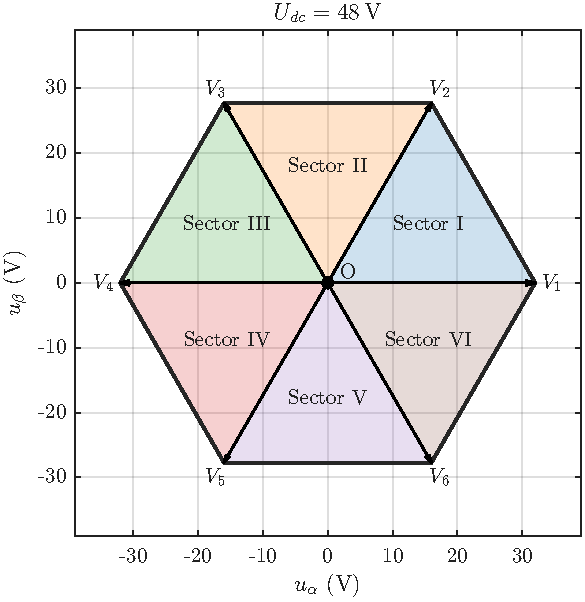
\includegraphics[width=0.72\textwidth]{svpwm_sector_distribution.pdf}
  \caption{SVPWM 六扇区与基本电压矢量分布图}
\end{figure}

图 1 展示了 SVPWM 六扇区与基本电压矢量在 $\alpha\beta$ 平面内的分布，且扇区边界每隔 $60^\circ$ 出现一次。只要参考电压位于正六边形内部，则后续求得的各段作用时间均为非负，系统处于线性调制区。

\subsection{作用时间定义与矩阵求解}

\begin{table}[!t]
  \centering
  \caption{六个扇区下 $T_0,T_1,T_2,T_7$ 关于 $u_\alpha,u_\beta$ 的表达式}
  \label{tab:svpwm-times}
  \renewcommand{\arraystretch}{1.35}
  \begin{tabularx}{\textwidth}{c >{\raggedright\arraybackslash}X}
    \toprule
    扇区  & 作用时间表达式                                                                                \\
    \midrule
    I   &
    $T_1 = \dfrac{\Ts}{\Udc}\!\left(\dfrac{3}{2}u_\alpha - \dfrac{\sqrt{3}}{2}u_\beta\right),\;
    T_2 = \dfrac{\sqrt{3}\Ts}{\Udc}u_\beta,$                                                     \\
        &
    $T_0 = T_7 = \dfrac{\Ts}{2} - \dfrac{\Ts}{4\Udc}\!\left(3u_\alpha + \sqrt{3}u_\beta\right).$ \\
    \midrule
    II  &
    $T_1 = \dfrac{\Ts}{\Udc}\!\left(\dfrac{3}{2}u_\alpha + \dfrac{\sqrt{3}}{2}u_\beta\right),\;
    T_2 = \dfrac{\Ts}{\Udc}\!\left(-\dfrac{3}{2}u_\alpha + \dfrac{\sqrt{3}}{2}u_\beta\right),$   \\
        &
    $T_0 = T_7 = \dfrac{\Ts}{2} - \dfrac{\sqrt{3}\Ts}{2\Udc}u_\beta.$                            \\
    \midrule
    III &
    $T_1 = \dfrac{\sqrt{3}\Ts}{\Udc}u_\beta,\;
    T_2 = \dfrac{\Ts}{\Udc}\!\left(-\dfrac{3}{2}u_\alpha - \dfrac{\sqrt{3}}{2}u_\beta\right),$   \\
        &
    $T_0 = T_7 = \dfrac{\Ts}{2} + \dfrac{\Ts}{4\Udc}\!\left(3u_\alpha - \sqrt{3}u_\beta\right).$ \\
    \midrule
    IV  &
    $T_1 = \dfrac{\Ts}{\Udc}\!\left(-\dfrac{3}{2}u_\alpha + \dfrac{\sqrt{3}}{2}u_\beta\right),\;
    T_2 = -\dfrac{\sqrt{3}\Ts}{\Udc}u_\beta,$                                                    \\
        &
    $T_0 = T_7 = \dfrac{\Ts}{2} + \dfrac{\Ts}{4\Udc}\!\left(3u_\alpha + \sqrt{3}u_\beta\right).$ \\
    \midrule
    V   &
    $T_1 = \dfrac{\Ts}{\Udc}\!\left(-\dfrac{3}{2}u_\alpha - \dfrac{\sqrt{3}}{2}u_\beta\right),\;
    T_2 = \dfrac{\Ts}{\Udc}\!\left(\dfrac{3}{2}u_\alpha - \dfrac{\sqrt{3}}{2}u_\beta\right),$    \\
        &
    $T_0 = T_7 = \dfrac{\Ts}{2} + \dfrac{\sqrt{3}\Ts}{2\Udc}u_\beta.$                            \\
    \midrule
    VI  &
    $T_1 = -\dfrac{\sqrt{3}\Ts}{\Udc}u_\beta,\;
    T_2 = \dfrac{\Ts}{\Udc}\!\left(\dfrac{3}{2}u_\alpha + \dfrac{\sqrt{3}}{2}u_\beta\right),$    \\
        &
    $T_0 = T_7 = \dfrac{\Ts}{2} - \dfrac{\Ts}{4\Udc}\!\left(3u_\alpha - \sqrt{3}u_\beta\right).$ \\
    \bottomrule
  \end{tabularx}
\end{table}

设一个开关周期为 $\Ts$。对于第 $s$ 个扇区，记两个相邻非零矢量 $\boldsymbol V(\theta_s)$ 与 $\boldsymbol V(\theta_s + \pi / 3)$ 的驻留时间分别为 $T_1$ 与 $T_2$，记两个零矢量 $\boldsymbol V_0$ 与 $\boldsymbol V_7$ 的驻留时间分别为 $T_0$ 与 $T_7$。则在一个开关周期内，SVPWM 满足平均伏秒关系
\[
  \boldsymbol u_s \Ts
  =
  T_1 \boldsymbol V(\theta_s)
  + T_2 \boldsymbol V\!\left(\theta_s + \frac{\pi}{3}\right)
  + T_0 \boldsymbol V_0
  + T_7 \boldsymbol V_7,
\]
本报告采用对称七段式，状态切换顺序为
\[
  \begin{aligned}
     & \boldsymbol V_0
    \rightarrow
    \boldsymbol V(\theta_s)
    \rightarrow
    \boldsymbol V\!\left(\theta_s + \frac{\pi}{3}\right)
    \rightarrow
    \boldsymbol V_7
    \rightarrow
    \boldsymbol V\!\left(\theta_s + \frac{\pi}{3}\right)
    \rightarrow
    \boldsymbol V(\theta_s)
    \rightarrow
    \boldsymbol V_0.
  \end{aligned}
\]
由此可得，对称七段式下零矢量时间满足
\[
  T_0 = T_7 = \frac{\Ts - T_1 - T_2}{2}.
\]

由于零矢量不产生 $\alpha\beta$ 平面内的输出分量，因此各扇区的平均伏秒方程可统一表示为
\[
  \boldsymbol u_s \Ts
  =
  T_1 \boldsymbol V(\theta_s)
  +
  T_2 \boldsymbol V\!\left(\theta_s + \frac{\pi}{3}\right).
\]
写成矩阵形式即
\[
  \begin{bmatrix}
    u_\alpha \\ u_\beta
  \end{bmatrix}\Ts
  =
  \underbrace{
    \frac{2}{3}\Udc
    \begin{bmatrix}
      \cos\theta_s & \cos\!\left(\theta_s + \frac{\pi}{3}\right) \\
      \sin\theta_s & \sin\!\left(\theta_s + \frac{\pi}{3}\right)
    \end{bmatrix}
  }_{\boldsymbol A_s}
  \begin{bmatrix}
    T_1 \\ T_2
  \end{bmatrix}.
\]
其中 $\boldsymbol A_s$ 为第 $s$ 个扇区对应的系数矩阵。

显然矩阵 $\boldsymbol A_s$ 在每个扇区内都可逆。于是可得到统一求解式
\[
  \begin{bmatrix}
    T_1 \\ T_2
  \end{bmatrix}
  =
  \Ts \boldsymbol A_s^{-1}
  \begin{bmatrix}
    u_\alpha \\ u_\beta
  \end{bmatrix}
  =
  \frac{\sqrt{3}\Ts}{\Udc}
  \begin{bmatrix}
    \sin\!\left(\theta_s + \frac{\pi}{3}\right) & -\cos\!\left(\theta_s + \frac{\pi}{3}\right) \\
    -\sin\theta_s                               & \cos\theta_s
  \end{bmatrix}
  \begin{bmatrix}
    u_\alpha \\ u_\beta
  \end{bmatrix}.
\]
表 \ref{tab:svpwm-times} 给出了六个扇区下 $T_0,T_1,T_2,T_7$ 关于 $u_\alpha,u_\beta$ 的显式表达式。


\section{指定工况下的时间曲线}


取 $dq$ 同步旋转坐标系下的参考电压分量为
\[
  U_{dc} = 48\,\mathrm{V},
  \qquad
  u_d = 0,
  \qquad
  u_q = 24\,\mathrm{V}.
\]
由逆 Park 变换可得
\[
  u_\alpha = -24 \sin\theta_e,
  \qquad
  u_\beta = 24 \cos\theta_e.
\]
此时参考矢量幅值恒为
\[
  \sqrt{u_\alpha^2 + u_\beta^2} = 24\,\mathrm{V}.
\]
又因为
\[
  \frac{\Udc}{\sqrt{3}} = \frac{48}{\sqrt{3}} \approx 27.71\,\mathrm{V},
\]
所以该工况始终位于 SVPWM 的线性调制区。


\begin{figure}[H]
  \centering
  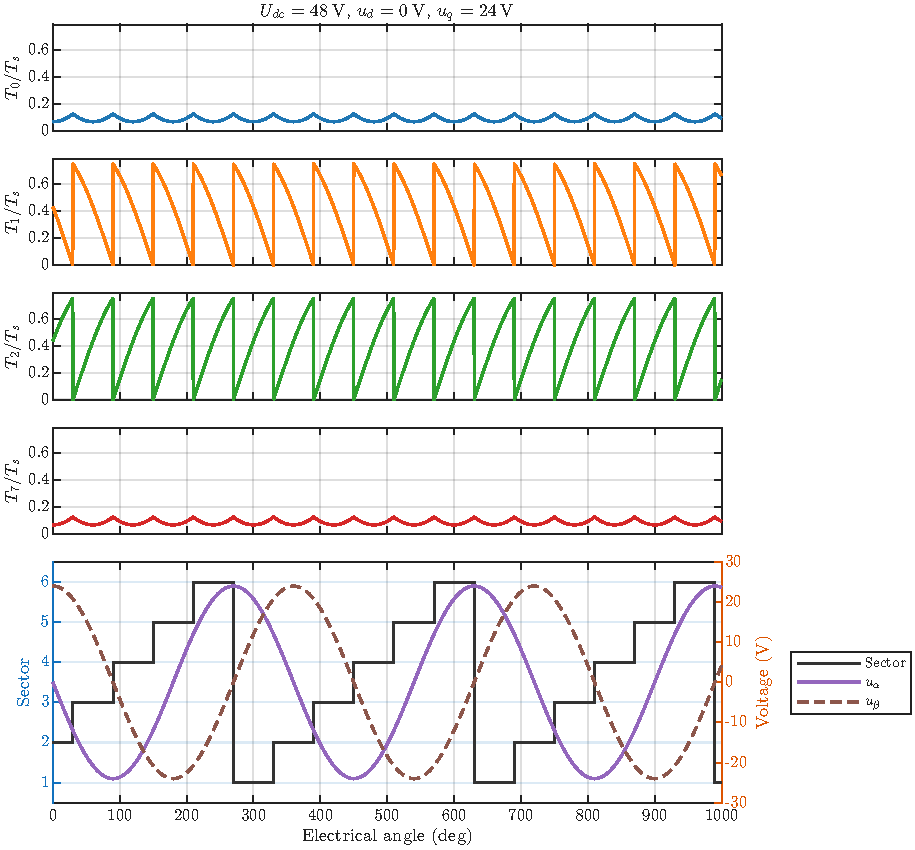
\includegraphics[width=0.96\textwidth]{svpwm_timing_curves.pdf}
  \caption{归一化作用时间与电压曲线}
\end{figure}

图 2 展示了 $U_{dc}=48\,\mathrm{V},\;u_d=0,\;u_q=24\,\mathrm{V}$ 条件下的归一化作用时间曲线。由该图可进一步观察到：
\begin{itemize}
  \item 由于采用对称七段式分配，始终有 $T_0 = T_7$，两条曲线完全重合；
  \item 随着电角度每跨越一个 $60^\circ$ 扇区边界，$T_1$ 与 $T_2$ 的角色互换，并在新扇区内重新开始一段分段正弦变化；
  \item $u_{\alpha}$ 和 $u_{\beta}$ 呈现相位相差 $90^\circ$ 的正弦波形，其组合后对应的电压矢量以固定幅值做圆周运动。
\end{itemize}

\appendix
\clearpage
\section{代码文件组织}

本次作业的 MATLAB 程序位于 \texttt{MATLAB\_workspace/hw12\_svpwm/}，各文件的功能见表 \ref{tab:hw12-files} 。

\begin{table}[H]
  \centering
  \caption{代码文件组织说明}
  \label{tab:hw12-files}
  \begin{tabularx}{\textwidth}{>{\raggedright\arraybackslash}p{0.37\textwidth} c >{\raggedright\arraybackslash}X}
    \toprule
    文件                                      & 类型   & 作用说明           \\
    \midrule
    \nolinkurl{hw12_svpwm_main.m}           & 入口脚本 & 主脚本            \\
    \nolinkurl{plotSvpwmSectorMap.m}        & 绘图函数 & 绘制六扇区与基本矢量分布图  \\
    \nolinkurl{plotSvpwmTimingCurves.m}     & 绘图函数 & 绘制时序曲线         \\
    \nolinkurl{+utils/createFigureA4.m}     & 辅助函数 & 创建统一尺寸的图窗      \\
    \nolinkurl{+utils/setDefaultGraphics.m} & 辅助函数 & 设置统一图形默认属性     \\
    \nolinkurl{+utils/tab10Color.m}         & 辅助函数 & 返回 Tab10 调色盘颜色 \\
    \bottomrule
  \end{tabularx}
\end{table}

\section{MATLAB 源码}

\subsection*{\texttt{hw12\_svpwm\_main.m}}
\VerbatimInput{../MATLAB_workspace/hw12_svpwm/hw12_svpwm_main.m}

\subsection*{\texttt{plotSvpwmSectorMap.m}}
\VerbatimInput{../MATLAB_workspace/hw12_svpwm/plotSvpwmSectorMap.m}

\subsection*{\texttt{plotSvpwmTimingCurves.m}}
\VerbatimInput{../MATLAB_workspace/hw12_svpwm/plotSvpwmTimingCurves.m}

\subsection*{\texttt{+utils/createFigureA4.m}}
\VerbatimInput{../MATLAB_workspace/+utils/createFigureA4.m}

\subsection*{\texttt{+utils/setDefaultGraphics.m}}
\VerbatimInput{../MATLAB_workspace/+utils/setDefaultGraphics.m}

\subsection*{\texttt{+utils/tab10Color.m}}
\VerbatimInput{../MATLAB_workspace/+utils/tab10Color.m}

\end{document}
